\section{Scan Konvertierung}

\subsection{Linie Rastern}

\textit{Eine Linie von $(x_0, y_0)$ nach $(x_1, y_1)$ rastern. Da in Pixel konvertiert werden muss. Methoden:}

\begin{itemize}
    \item \textit{Brute Force; über jeden Pixel und runden}
    \item \textit{Brute Force inkrementell (DDA = Digital Differential Analyzer); $y_{i+1} = m * x_{i+1) + B = y_i + m}$,
          Nachteil Gleitkommazahlen und Runden (aufwändig)}
    \item \textit{Mittelpunktschema; Nächsten Punkt wird Kalkuliert durch if / else}
\end{itemize}

\subsection{Mittelpunktschema}
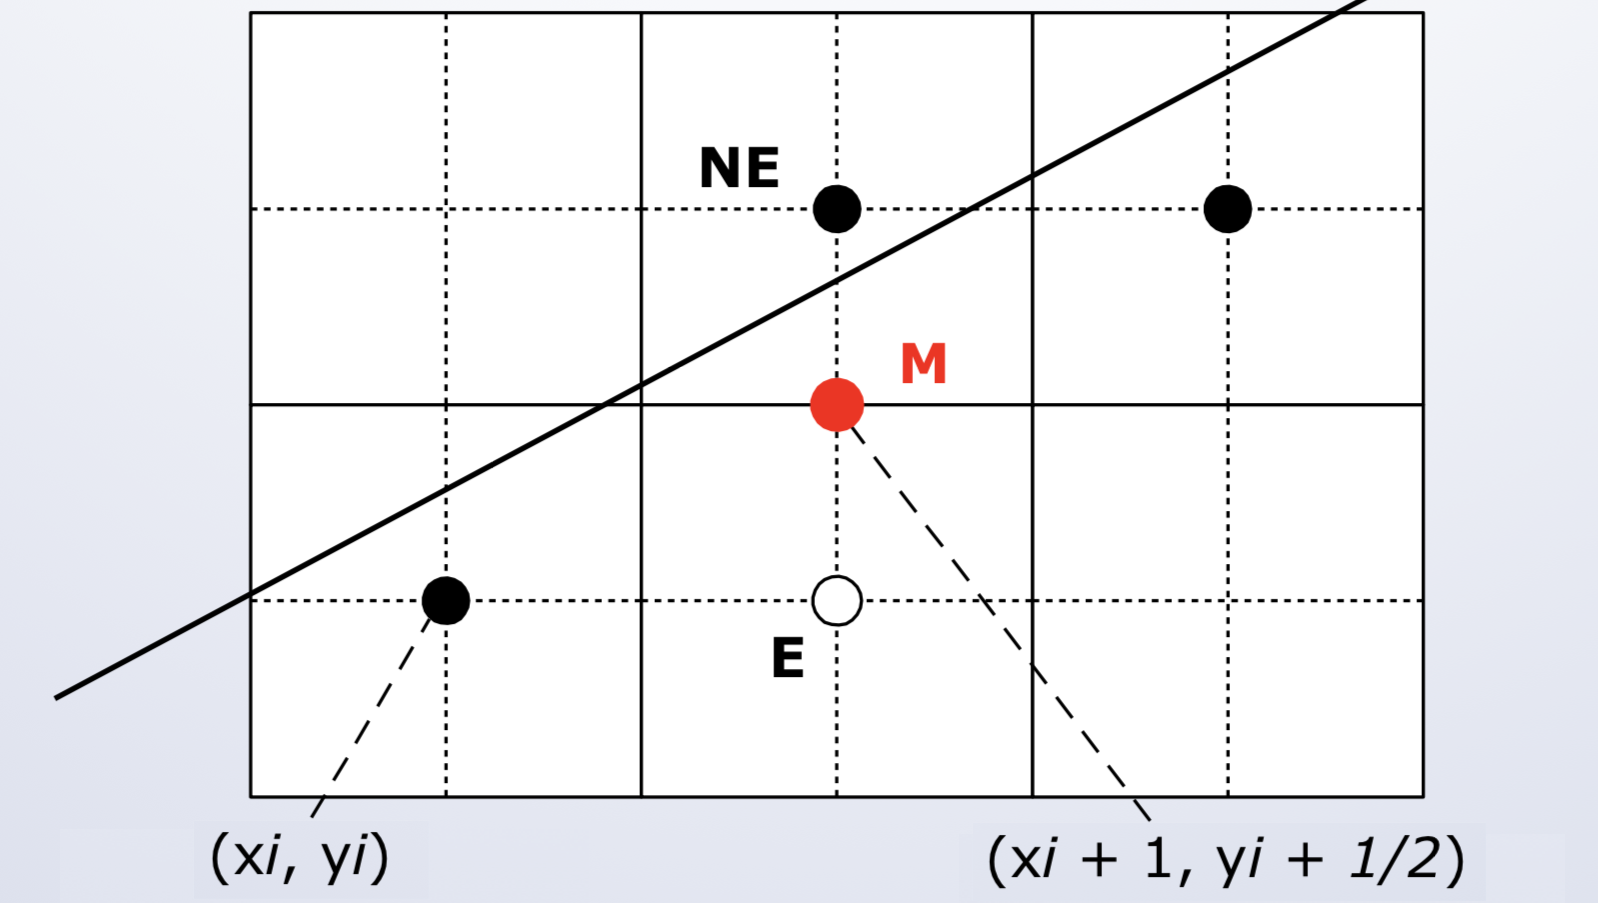
\includegraphics[width=0.35\textwidth]{assets/Mittelpunktschema.png}

\textit{Ist eine inkrementelle methode zum Rastern. Mittelpunkt
wird betrachtet um nächsten Punkt zu finden. ($M = (x_i+1, y_i+\frac{1}{2})$, $E = (x_i+1, y_i)$, $NE = (x_i+1, y_i+1)$)}\\

Initialisierung:\\
$D_x = x_1 - x_0$; \\
$D_y = y_1 - y_0$; \\
$D_E = 2 * D_y$; \\
$D_{NE} = 2 * (D_y - D_x)$; \\
$d = 2*D_y - D_x$; \\
$y = y_0$ \\

\textit{Wegen 1/2 alles mal 2, damit gerade Zahlen}

\textit{
    Für jeden nächsten $d$ Wert, wenn $d <= 0$,
    dann $d = d + D_{NE}$ ansonsten $d = d + D_{NE}$ und $y$ inkremenrieren.
    Jeweils den Punkt $P(x,y)$ zeichnen. $x$ jedesmal inkrementieren.
}

Berechnung:
\begin{lstlisting}
WritePixel(x0, y0)
for x = x0+1 to x1 do
  if d <= 0 then
    d = d + DE;
  else
    d = d + DNE;
    y = y + 1;
  end
  WritePixel(x,y);
end
\end{lstlisting}

\subsection{Kreis Rastern}

\textit{Selbe Methode wie bei den Linien kann für Kreise angewendet werden.}

\subsection{Mittelpunktschema Kreis}

\textit{Funktion für Kreis: $F(x,y) = x^2 + y^2 - R^2$}\\

$x = 0$\\
$y = R$\\
$d = 1 - R$\\
$D_{E} = 2*x + 3$\\
$D_{NE} = 2*(x-y)d + 5$\\

\textit{
    Für jeden nächsten $d$ Wert wiederholen bis $y > x$, wenn $d < 0$,
    dann $d = d + D_{E}$ ansonsten $d = d + D_{NE}$ und $y$ dekrementieren.
    Jeweils den Punkt $P(x,y)$ zeichnen. $x$ jedesmal inkrementieren.
}

\begin{lstlisting}
WritePixel(x,y);
while y > x do
  if d < 0 then
    d = d + 2*x + 3;
  else
    d = d +2*(x-y) + 5;
    y = y - 1;
  end
  x = x + 1;
  WritePixel(x,y);
end
\end{lstlisting}

\subsection{Regionen füllen}

\textit{Entweder durch 4-er oder 8-er Zusammenhang definiert}

\begin{tabular}{cl}
    \multirow{3}{*}{
        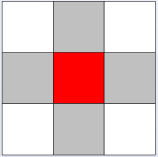
\includegraphics[width=0.05\textwidth]{assets/region-filling-4.png}
    } & \\
    & \textit{4-er Zusammenhang} \\
    & \\
\end{tabular}
\begin{tabular}{cl}
    \multirow{3}{*}{
        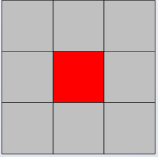
\includegraphics[width=0.05\textwidth]{assets/region-filling-8.png}
    } & \\
    & \textit{8-er Zusammenhang} \\
    & \\
\end{tabular}

\subsubsection{FloodFill}

\textit{Füllen durch selben abfrage ob selbe Farbe (Photoshop Zauberstab)}
\begin{lstlisting}
proc FloodFill(int x, int y,
Color oldColor, Color newColor)
  if ReadPixel(x,y) == oldColor then
    WritePixel(x,y,newColor);
    FloodFill(x, y-1, oldColor, newColor);
    FloodFill(x-1,y, oldColor, newColor);
    FloodFill(x, y+1, oldColor, newColor);
    FloodFill(x+1, y, oldColor, newColor);
  end
end
\end{lstlisting}

\subsection{Zeichnen von gefüllten Polygonen}

\subsubsection{Scanlinien Algorithmus}

\begin{tabular}{cc}
  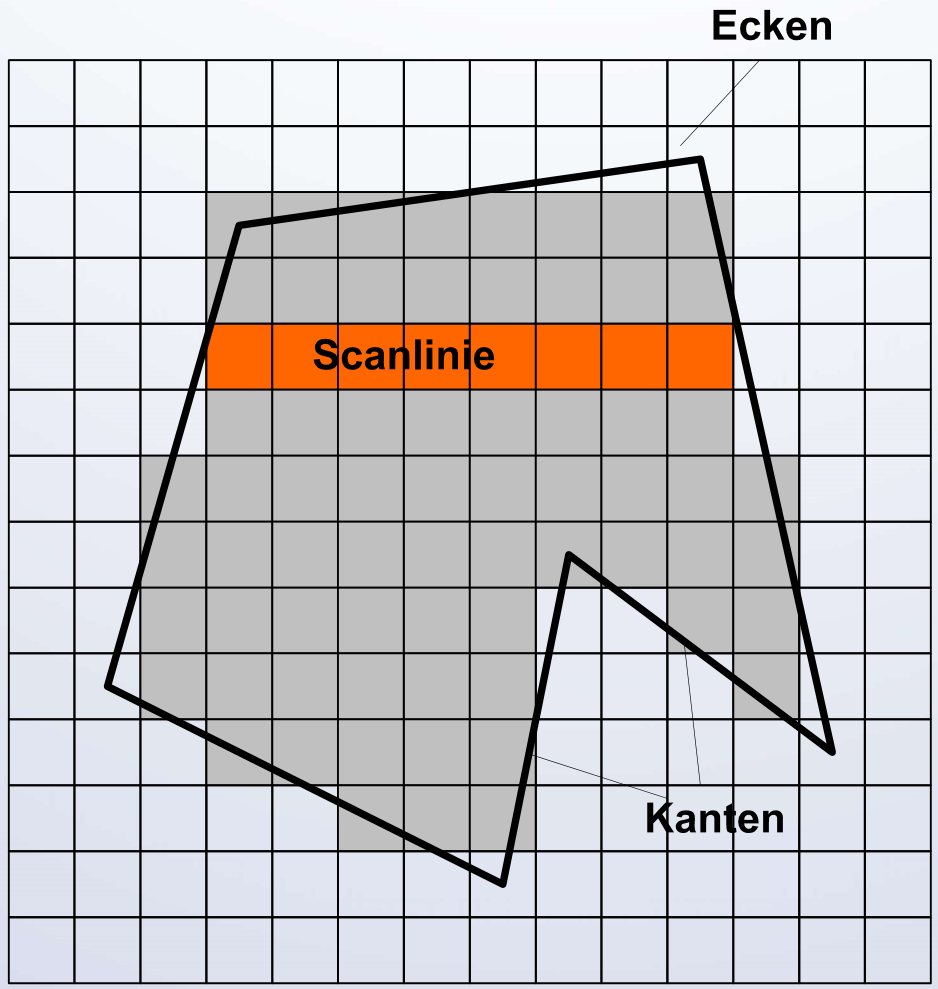
\includegraphics[width=0.25\textwidth]{assets/scanlinien-alg.png} &
  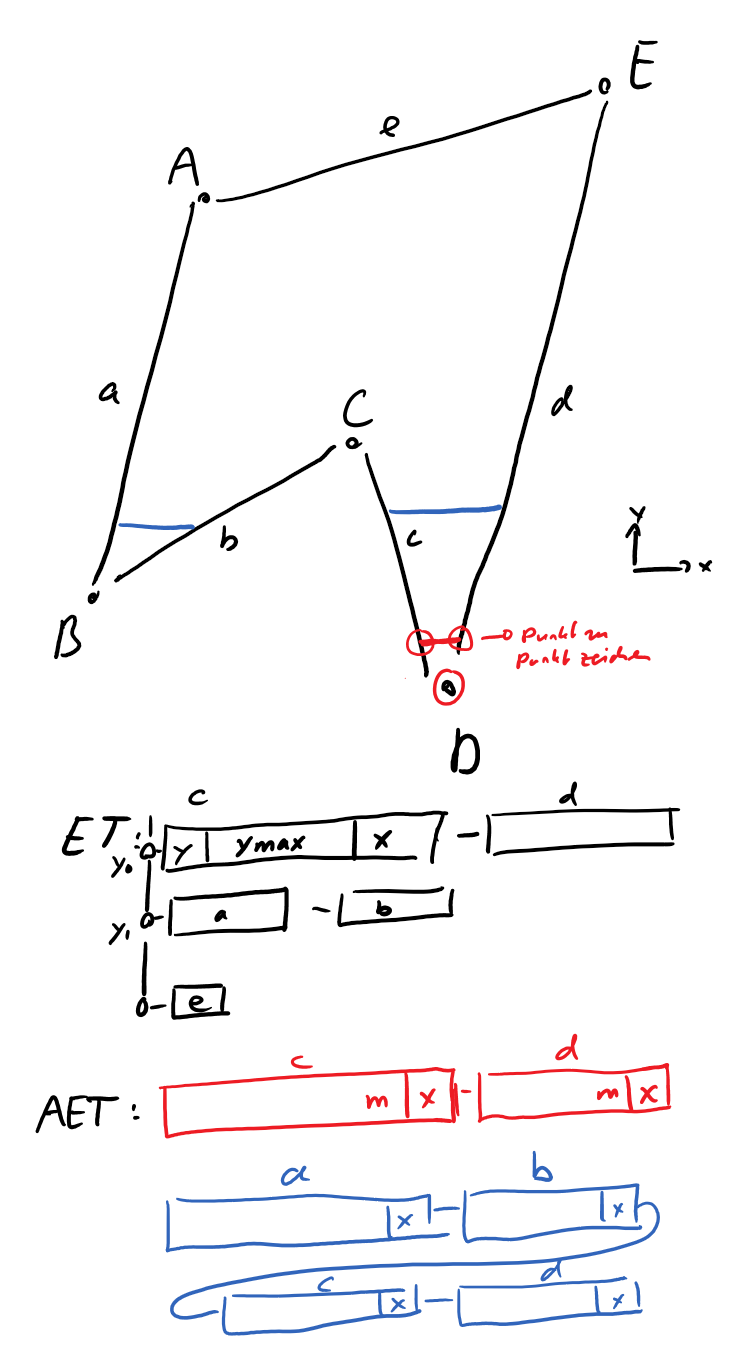
\includegraphics[width=0.25\textwidth]{assets/scanlinien-alg-demo.png} \\
\end{tabular}

\begin{itemize}
	\item Zeilenweise färben (Spans entlang der y Koordinate -> Scanlinien)
	\item Kantentabelle (edgetable ET)\\
    sortierte Kanten (Linien) des Polygon nach min y (innerhalb davon nach max x)
  \item Einträge werden gespeichert durch $[x|1/m|y_{min}|y_{max}]$
	\item Tabelle aktiver Kanten (AET)\\
		Momentane Kanten für Scanlinie (sortiert nach x asc) zum Zeichnen vom einer Kante zur nächsten (immer zwei)
\end{itemize}

\begin{lstlisting}
Erzeuge ET (Kantentabelle)
Initialisiere AET = empty  (Aktive Kanten)
y=0
repeat
  Addiere und entferne alle Kanten
      ET(y) zu AET
  Sortiere AET nach x
  Zeichne Spans
  y=y+1
  Entferne Kanten mit ymax = y aus AET
  Aktualisiere den x Wert aller
      Kanten in AET
until AET == empty and ET == empty
\end{lstlisting}

\subsubsection{Zeichnen von Dreiecken}

\textit{Brute Force: Alle Pixel probieren, ob im Dreieck}

\begin{tabular}{cl}
  \multirow{3}{*}{
      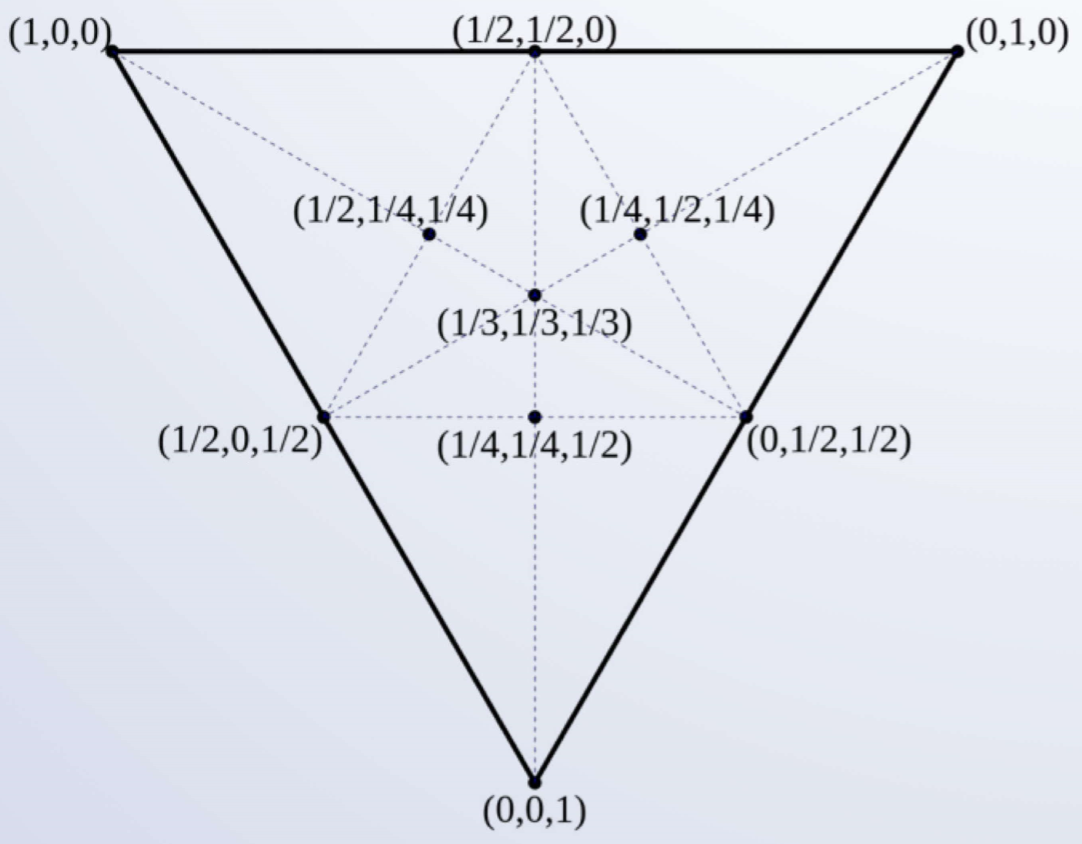
\includegraphics[width=0.2\textwidth]{assets/draw-baryzentrische-coordinates.png}
  } & \\
  & Baryzentrische Koordinaten \\
  & \\
  & $P = \alpha A + \beta B + \gamma C$\\
  & \\
  & $\alpha+\beta+\gamma =1$\\
  & \\
\end{tabular}

\textit{Wenn Werte zwischen 0 und 1, dann ist Punkt P innerhalb von ABC.
Wert einer Koordinate entspricht dem Verhältnis der Fläche eines Teildreiecks
mit Ecke P zur Fläche von ABC}\\

\begin{tabular}{cl}
  \multirow{3}{*}{
    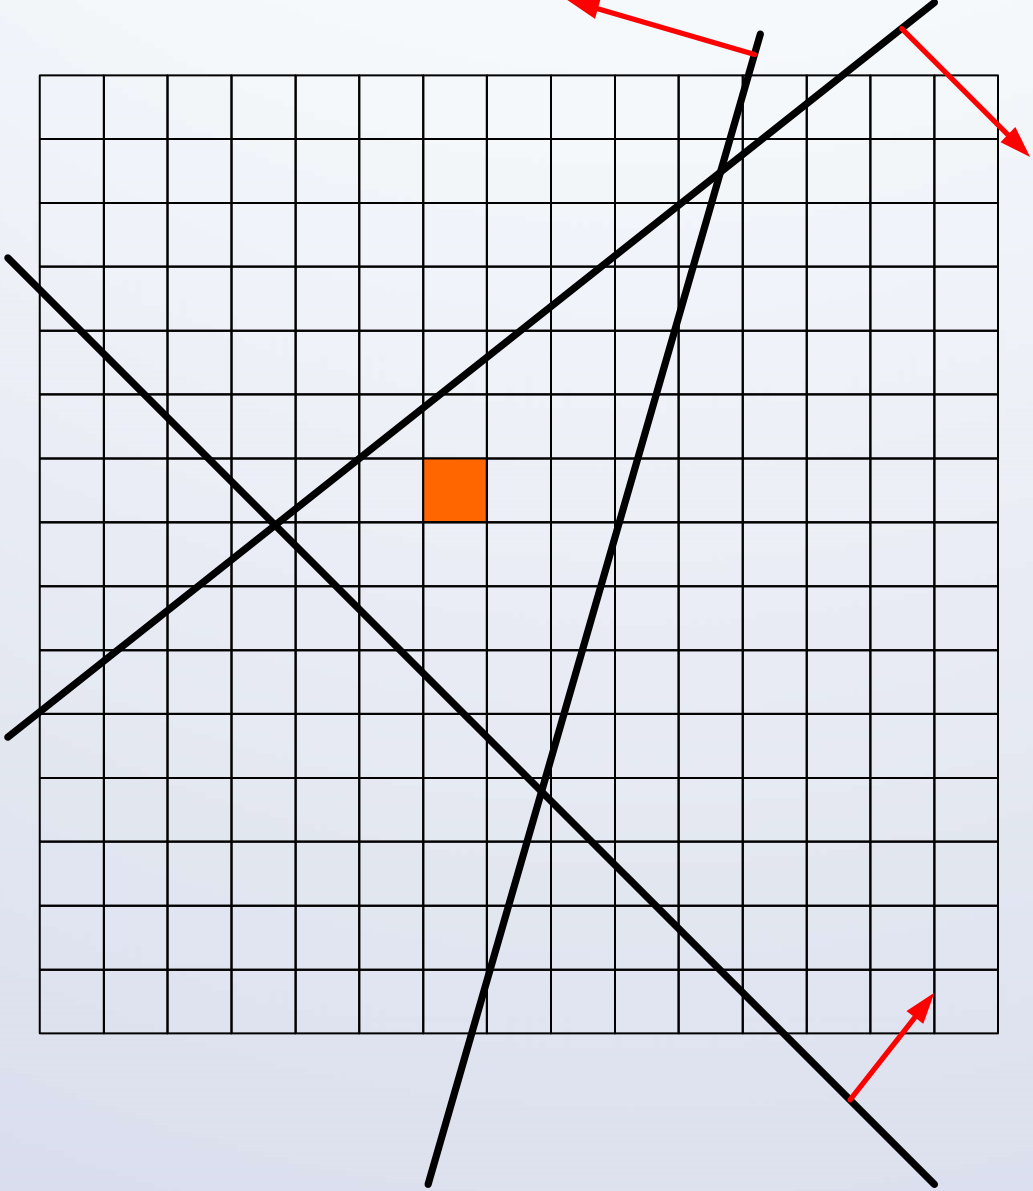
\includegraphics[width=0.15\textwidth]{assets/draw-line-side.png}
  } & 2. Bruteforce Option \\
  & \\
  & Unterteilung in 3 Geraden. \\
  & Zeichnen wenn auf der richtigen\\
  & Seite aller Geraden \\
  & \\
  & \\
\end{tabular}

\subsection{Anti-Aliasing}
\textit{Treppenmuster vermeiden}
\begin{itemize}
	\item Prefiltering -> Farbintensität proportional zur Fläche oder Linie
  \item Supersampling -> Bild mit höherer Auflösung berechnen und Farbmittelwerte
    als Übergänge zeichnen (4x Sample Patter, Quincunx AA Sample Pattern)
\end{itemize}
